\documentclass[../../main.tex]{subfiles}

\graphicspath{{../../fig/}}
\setcounter{section}{0}

\begin{document}
\chapter{重力参照計の評価}
\ref{}にて述べたように、本較正装置では重力参照計を用いて絶対角度を測定するが、
これまでに使用が想定されていた Digi-Pas 社製の DWL5000-XY は要求性能を満たさなかった。
今回、新たに候補となった Sherborne Sensors 社製の DSIC-2051-60 を評価した。
本章では、はじめに要求精度と評価すべき項目について確認したのち、
新しい重力参照計の概要の共有、各評価項目の手法と結果について述べる。
\section{要求精度と評価項目}
要求される精度は、表\ref{}中にある値から合計誤差が $\delta\theta < 0.1\tcdegree$ となることであり、
式\ref{}中の $\theta_{\mathrm{sens}}$ にして $\delta\theta_{\mathrm{sens}}<0.06\tcdegree$ である。
これを重力参照計の要求精度に換算する。
式\eqref{}より、重力参照計の各 $X$ 軸、$Y$ 軸の誤差を $\delta\theta_{X},\,\delta\theta_{Y}$ とすると、
$\theta_{\mathrm{sens}}$ の誤差 $\delta\theta_{\mathrm{sens}}$ は
\begin{align}
    \delta\theta_{\mathrm{sens}} &= 
        \sqrt{\qty(\dfrac{\sin\beta}{\sin^2\alpha+\sin^2\beta} \delta\qty(\sin\alpha))^2 + \qty(\dfrac{\sin\alpha}{\sin^2\alpha+\sin^2\beta} \delta\qty(\sin\beta))^2}\\ 
    \delta\qty(\sin\alpha) &= \sqrt{\qty(\dv{\sin\alpha}{\theta_X}\delta\theta_X)^2+\qty(\dv{\sin\alpha}{\theta_Y}\delta\theta_Y)^2}\\
    \delta\qty(\sin\beta) &= \sqrt{\qty(\dv{\sin\beta}{\theta_X}\delta\theta_X)^2+\qty(\dv{\sin\beta}{\theta_Y}\delta\theta_Y)^2} \\
    \dv{\sin\alpha}{\theta_X} &= \cos\theta_{\mathrm{slope}1}\cos\theta_X - \sin\theta_{\mathrm{slope}1}\sin\theta_{\mathrm{slope}2}\dfrac{\sin\theta_X\cos\theta_X}{\sqrt{1-\sin^2\theta_X-\sin^2\theta_Y}} \\
    \dv{\sin\alpha}{\theta_Y} &= -\sin\theta_{\mathrm{slope}1}\cos\theta_{\mathrm{slope}2}\cos\theta_Y - \sin\theta_{\mathrm{slope}1}\sin\theta_{\mathrm{slope}2}\dfrac{\sin\theta_Y\cos\theta_Y}{\sqrt{1-\sin^2\theta_X-\sin^2\theta_Y}} \\
    \dv{\sin\beta}{\theta_X} &= \sin\theta_{\mathrm{slope}1}\cos\theta_X + \cos\theta_{\mathrm{slope}1}\sin\theta_{\mathrm{slope}2}\dfrac{\sin\theta_X\cos\theta_X}{\sqrt{1-\sin^2\theta_X-\sin^2\theta_Y}} \\
    \dv{\sin\beta}{\theta_Y} &= \cos\theta_{\mathrm{slope}1}\cos\theta_{\mathrm{slope}2}\cos\theta_Y + \cos\theta_{\mathrm{slope}1}\sin\theta_{\mathrm{slope}2}\dfrac{\sin\theta_Y\cos\theta_Y}{\sqrt{1-\sin^2\theta_X-\sin^2\theta_Y}}
\end{align}
のように表される。
$\theta_{\mathrm{slope}1}=210\tcdegree,\,\theta_{\mathrm{slope}2}=40\tcdegree$ は\ref{subsubsec:wg_tiltsensor_slope}にて導入したスロープの角度である。
重力参照計の両軸ともに同程度の誤差を持つと仮定し、スロープの角度から生じる誤差を無視すると、およそ $\delta\theta_{X} \sim \delta\theta_{Y} \leq 0.04\tcdegree$ が要求精度となる。

\colortext{blue}{いい文章が思いつかないなぁ。}
観測サイトはその気温が $\SI{-15}{\degreeCelsius} \sim \SI{20}{\degreeCelsius}$ と変動する過酷な環境である。
\begin{itemize}
    \item 電源の入れ直しによるオフセットの変動
    \item 観測サイトの環境 $\SI{-15}{\degreeCelsius} \sim \SI{20}{\degreeCelsius}$ にて、温度変動による出力の変動
\end{itemize}
となる。

\section{重力参照計の概要}
図\ref{}に重力参照計の外観を示す。図中の $X$ 軸、$Y$ 軸と水平面。
\begin{figure}
    \centering
    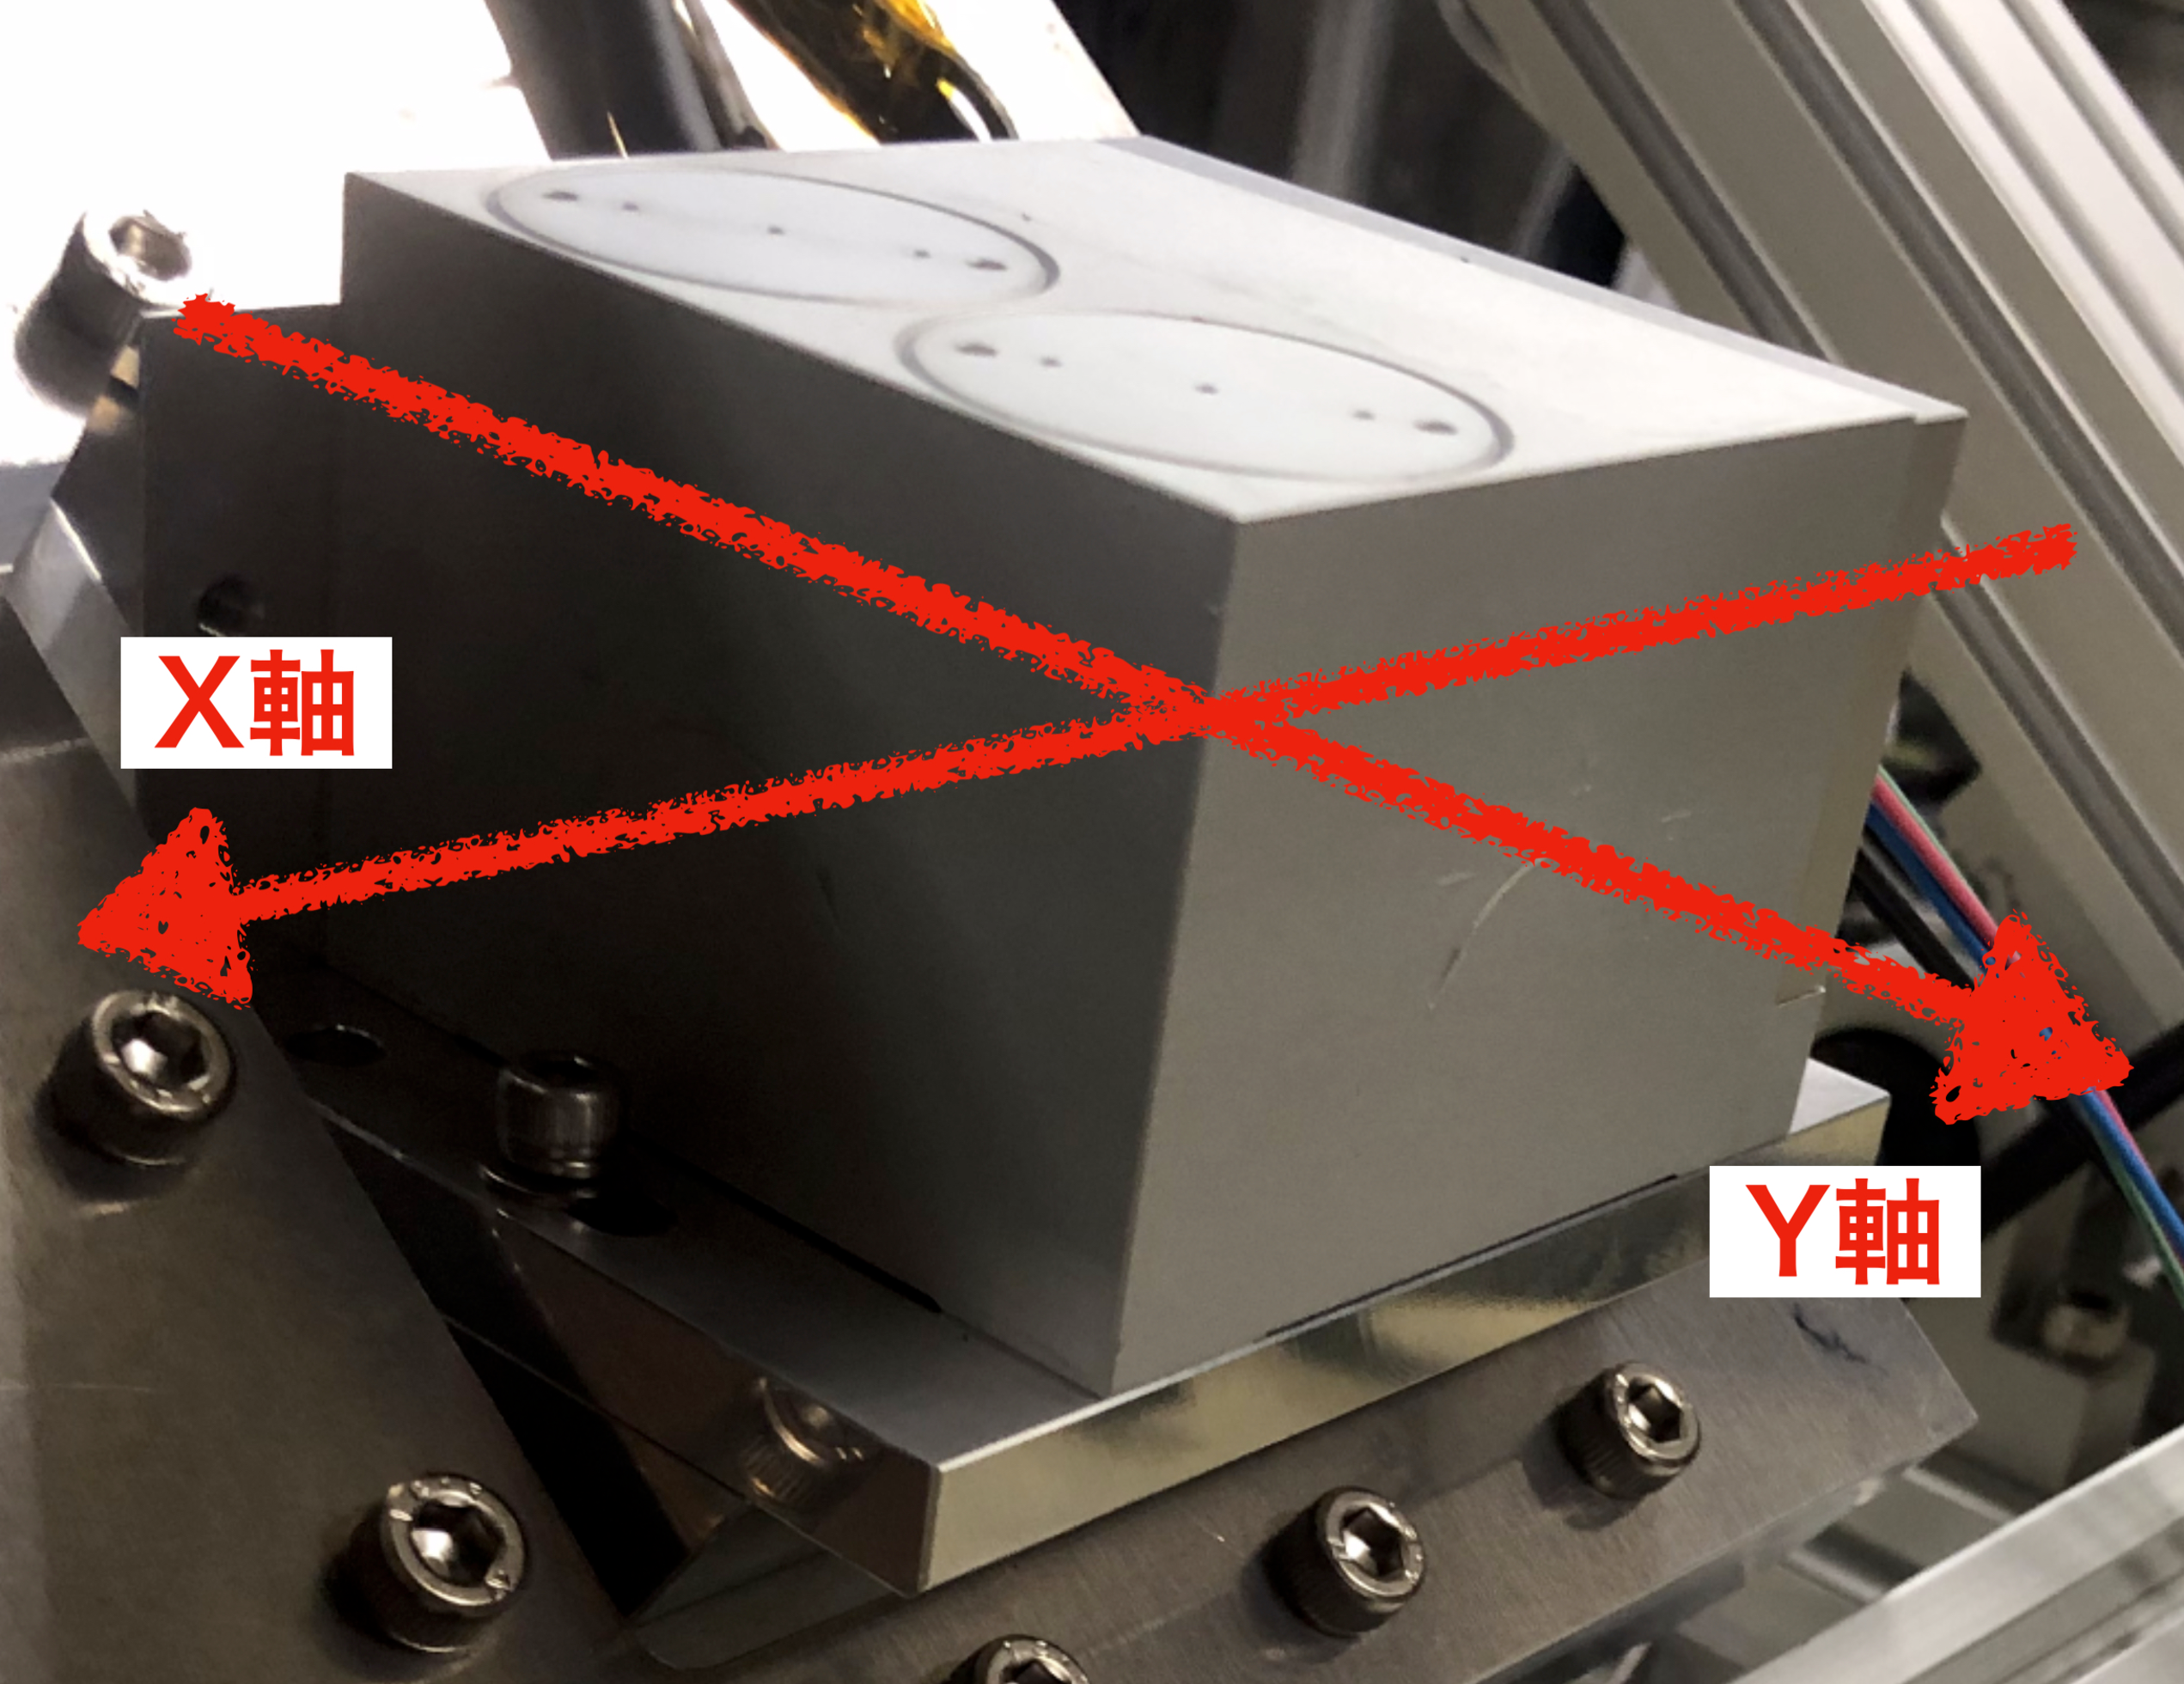
\includegraphics[width=0.5\textwidth]{tiltsensor/tiltsensor_overview.pdf}
    \figcaption{Sherborne Sensors 社製 DSIC-2051-60 の外観}
    \label{fig:tiltsensor_DSIC-2051-60}
\end{figure}
\section{電源の入れ直しによるオフセット変動の評価}
\subsection{評価系}
\subsection{測定結果}
\section{温度による出力の変化の評価}
\subsection{評価系の概要}
\subsection{測定結果}
\subsection{測定結果の考察}
\subsection{まとめ}
\end{document}